\exo{Lecture graphique (graphe page \pageref{fonction})}


\begin{figure}
\begin{center}
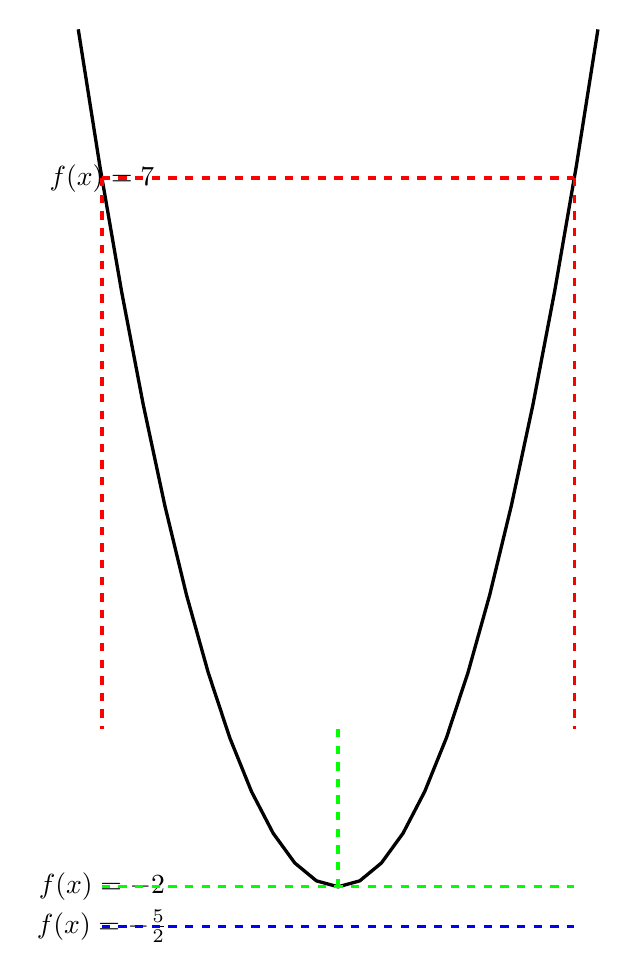
\begin{tikzpicture}
\tkzInit[xmin=-2.3,xmax=4.3,ymin=-3,ymax=9]
\tkzGrid[sub,color=gray, subxstep=.5,subystep=.5]
\tkzAxeXY[very thick]
\tkzGrid

\draw [domain=-2.3:4.3, very thick,] plot(\x,{(\x)^2 - 2*\x - 1});

\correction{\draw (-2,7) node {$f(x) = 7$};
\draw (4,7) node {};
\draw (-2,0) node {};
\draw (4,0) node {};

\draw [very thick, dashed, red] (-2,7) -- (4,7);
\draw [very thick, dashed, red] (-2,7) -- (-2,0);
\draw [very thick, dashed, red] (4,7) -- (4,0);

\draw (-2,-2) node {$f(x) = -2$};
\draw [very thick, dashed, green](-2,-2) -- (4,-2);
\draw [very thick, dashed, green](1,-2) -- (1,0);


\draw (-2,-2.5) node {$f(x) = -\frac{5}{2}$};
\draw [very thick, dashed, blue](-2,-2.5) -- (4,-2.5);}

\end{tikzpicture}
\end{center}
\caption{Courbe $\mathcal{C}_f$, représentative de la fonction $f:x\longmapsto x^2-2x-1$}
\label{fonction}
\end{figure}



\question{Résoudre graphiquement (on pourra rendre l'énoncé avec les traits de construction):}

\subquestion{}
$f(x) = 7$

\correction{

}

\subquestion{}
$f(x) = -2$

\correction{

}

\subquestion{}
$f(x) = -\frac{5}{2}$

\correction{

}

\question{Retrouver les résultats de la question précédente par le calcul}

\correction{

\begin{itemize}
 \item $f(x) = 7 \Leftrightarrow x^2 - 2x - 8 = 0$. $\Delta = 36 > 0$

L'équation a donc 2 solutions:  $x_{1,2} = \dfrac{-b \pm \sqrt{\Delta}}{2a}$

$x_1 = \frac{2+6}{2} = 4$

$x_2 = \frac{2-6}{2} = -2$

On a donc: \Answer{$\mathcal{S} = \left\lbrace -2 ; 4 \right\rbrace$}

\item $f(x) = -2 \Leftrightarrow x^2 - 2x + 1 = 0$. $\Delta = 0$

L'équation a donc 1 solution:  $x_{1} = \dfrac{-b }{2a}$

$x_1 = \frac{2}{2} = 1$

On a donc: \Answer{$\mathcal{S} = \left\lbrace 1 \right\rbrace$}

    \item $f(x) = -\frac{5}{2} \Leftrightarrow x^2 - 2x + \frac{3}{2} = 0$. $\Delta = -2 < 0$

L'équation n'a donc pas de solution: \Answer{$S = \emptyset $}
\end{itemize}


}
